\speaker{\Michel}

\begin{frame}
\frametitle{\underline{M}VC : Le modèle}
\begin{figure}[!h]
	\begin{center}
	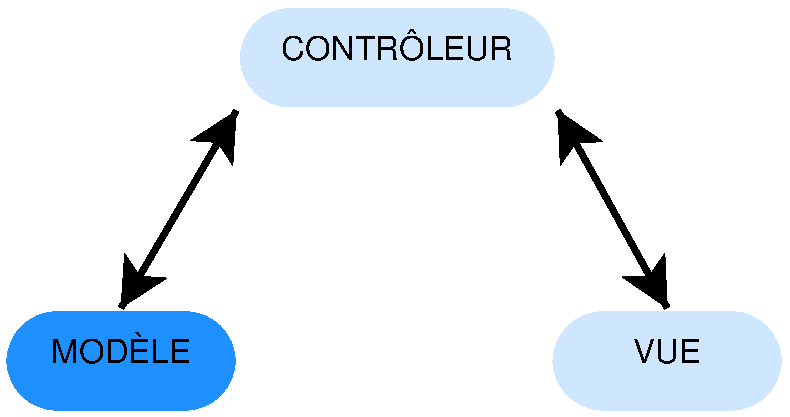
\includegraphics[scale=0.5]{images/mvcModele}
	\caption{Architecture \underline{M}VC}
	\end{center}
\end{figure}
Modèle :  ptite def simpliste
\end{frame}

\begin{frame}
	\frametitle{\underline{M}VC : Le modèle}
	\begin{block}{Partie wesh méga importante }
		
	
		Super important, karément long deux grosses parties :
		\begin{itemize}
			\item Ke c'était long de faire le diagramme 
			\item L'implémentation de la BD kon a eu deux choix kon voit après !!
		\end{itemize}
	\end{block}
\end{frame}

\begin{frame}
	\frametitle{\underline{M}VC : Le modèle}
	\begin{block}{Création de la BD et communication aevc notre framework et l'orm Doctrine}
		
		exploration de deux choix possibles = tel solution proposée
		\begin{itemize}
			\item Top Down -> def on part du haut on descend = langage objet création des tables en BD
			\item Buttom - Up -> def : inverse top down, part dans bas pour aller en haut = création table => création objet
		\end{itemize}
	\end{block} 
\end{frame}

\speaker{\Julie}
\begin{frame}
	\frametitle{\underline{M}VC : Le modèle}
	\begin{block}{Top down}
		Pourquoi c'est kool
		\begin{itemize}
			\item rapide ?
			\item C'est la mode ?
		\end{itemize}
 
		Pourquoi c'est pas cool
		\begin{itemize}
			\item cracra -> modeler à partir de ça
		\end{itemize}
	\end{block}
\end{frame}


\begin{frame}
	\frametitle{\underline{M}VC : Le modèle}
	\begin{block}{Bottom up}
	Pourquoi c'est kool
		\begin{itemize}
			\item propre
			\item a
		\end{itemize} 
		Pourquoi pas cool
		\begin{itemize}
			\item chronophage
			\item a
		\end{itemize}
	\end{block}
  
\end{frame}

\begin{frame}
	\frametitle{\underline{M}VC : Le modèle}
	\begin{block}{Choix}
		Blabla c'est mieux Bottum up !
		dixit dorianne : "perdre du temps pour faire mieux" , meilleur choix, blabla maintenabilité responsive des conneries quoi
	\end{block}
\end{frame}